\documentclass[conference]{IEEEtran}
% Add the compsoc option for Computer Society conferences.
%
% If IEEEtran.cls has not been installed into the LaTeX system files,
% manually specify the path to it like:
% \documentclass[conference]{../sty/IEEEtran}





% *** Do not adjust lengths that control margins, column widths, etc. ***
% *** Do not use packages that alter fonts (such as pslatex).         ***
% There should be no need to do such things with IEEEtran.cls V1.6 and later.
% (Unless specifically asked to do so by the journal or conference you plan
% to submit to, of course. )


% correct bad hyphenation here
\hyphenation{op-tical net-works semi-conduc-tor}
\usepackage{graphicx}
\usepackage{balance}  % for  \balance command ON LAST PAGE  (only there!)
\usepackage{array}
\usepackage{xspace}
\usepackage{hyperref}
\usepackage{array}
%\usepackage{booktabs}
%\usepackage{color}
%\usepackage{algorithmic}
%\usepackage{algorithm}
%\usepackage[table,xcdraw]{xcolor}
%\usepackage{epsfig}
%\usepackage{epstopdf}
%\usepackage{subfigure}
%\usepackage[english]{babel}
\usepackage{multirow}
\usepackage{amsmath}
%\usepackage{caption}

\begin{document}


\title{Ring: Real-Time Emerging Event Monitoring over Text Stream}

%\author{\IEEEauthorblockN{Michael Shell}
%\IEEEauthorblockA{School of Electrical and\\Computer Engineering\\
%Georgia Institute of Technology\\
%Atlanta, Georgia 30332--0250\\
%Email: http://www.michaelshell.org/contact.html}
%\and
%\IEEEauthorblockN{Homer Simpson}
%\IEEEauthorblockA{Twentieth Century Fox\\
%Springfield, USA\\
%Email: homer@thesimpsons.com}
%\and
%\IEEEauthorblockN{James Kirk\\ and Montgomery Scott}
%\IEEEauthorblockA{Starfleet Academy\\
%San Francisco, California 96678-2391\\
%Telephone: (800) 555--1212\\
%Fax: (888) 555--1212}}

% for over three affiliations, or if they all won't fit within the width
% of the page, use this alternative format:
%
\author{\IEEEauthorblockN{
Weiren Yu,
Jianxin Li,
Richong Zhang,
Shuai Ma,
Jinpeng Huai
}
\IEEEauthorblockA{
SKLSDE Lab, Beihang University, Beijing, China\\
\{yuwr, lijx zhangrc\}@act.buaa.edu.cn,
\{mashuai, huaijp\}@buaa.edu.cn}

}



\maketitle

\newcommand{\eat}[1]{}
\newcommand{\un}[1]{\underline{#1}}
\newcommand{\ring}{{\sc Ring}\xspace}
\newcommand{\ie}{\emph{i.e.,}\xspace}
\newcommand{\eg}{\emph{e.g.,}\xspace}


\begin{abstract}
In this paper, we demonstrate \href{http://ring.cnbigdata.org}{\ring}\footnote{http://ring.cnbigdata.org},
a \un{R}eal-t\un{i}me emerging eve\un{n}t monitorin\un{g} system over microblog text streams.
\ring is the first system to integrate efforts from both event analysis research and system research and present several advantages over existing methods
\cite{xie2014clear, schubert2014signitrend, mathioudakis2010twittermonitor}.
From a semantic perspective,
(1) \ring detects emerging events at an early stage at multiple time scales even with small magnitude of traffic by adopting anomaly detection method.
(2) \ring is the first to discover fine-granularity hierarchies of sub-events in a streaming setting for emerging events analysis.
(3) \ring can trace the evolution of events at multiple time scales using various metrics of similarity.
A refinement procedure is performed to filter out spam events and provide contextual information.
From a system perspective,
(1) \ring optimizes time-ranged keyword query for improved efficiency of user interactivity and event evolution tracking.
(2) \ring implements its graph stream model on Spark and improves the incremental update efficiency of the platform.
\ring also provides a friendly and highly interactive user interface to visualize events and statistics.

%\ring is a promising system that provides real-time comprehensive event analysis and user-friendly interface
%to facilitate the analysis of trending events.
\end{abstract}
% IEEEtran.cls defaults to using nonbold math in the Abstract.
% This preserves the distinction between vectors and scalars. However,
% if the conference you are submitting to favors bold math in the abstract,
% then you can use LaTeX's standard command \boldmath at the very start
% of the abstract to achieve this. Many IEEE journals/conferences frown on
% math in the abstract anyway.


\IEEEpeerreviewmaketitle



\section{Introduction}

Emerging event monitoring over microblog platforms attracts much attention in both research and application due to the real-time nature and viral diffusion of information.
In fact they have many times been the first reporter or even the major hosting venue of significant events, such as earthquake forecast or a presidential election.
A wide variety of events would emerge from such platforms, ranging from political and daily affairs to natural disasters and public security menace.
Not only are the events that attract mass attention important, but also those events with great potential to go viral while only drew attention from a small fraction of users, \eg a road stabbing with growing witnesses tweeting about it.
Despite the versatility in topics and traffic, different aspects of events and different angles of user descriptions would complement each other.
Further insights could be revealed from hierarhical information such as causality of events, \eg the capture of a criminal and the crime he had committed, or categorical information \eg different genres of news from the same agency.
What's more, trends would emerge from different time granularities from minutes to hours, \eg a concert or sports game, or even days to months, \eg a publicly concerned long trial.
The temporal evolution pattern could be retrieved to get the big picture of events.
Emerging event monitoring, \ie early detection, hierarchical correlation analysis, and temporal evolution tracking of these events in real-time, provide valuable insights and allow timely response to these events.
Such intelligence are desirable and directly related to government agencies, news groups and marketing strategies, etc.

However, traditional topic modeling methods (e.g. Latent Dirichlet Allocation%~\cite{blei2003latent}
) and its derivatives could not be directly applied to noisy short texts nor could they perform early detection of emerging events in real-time.
TwitterMonitor~\cite{ mathioudakis2010twittermonitor} provide online detection for general trending events but could not reveal multiple aspects of events nor track the evolution of them.
CLEar~\cite{xie2014clear} can provide real-time event detection and tracking but could not provide hierarchical analysis of events.
Neither of them could identify potential viral events at small scale.
Signitrend~\cite{schubert2014signitrend} could detect potential viral events at small scale but confined to detection and could not provide event correlation analysis.
The method would also tend to generate trends that only contain a single keyword, which is hard to comprehend for users.
Another important aspect of an interactive real-time emerging event monitoring application is system optimization. 
None of these above methods or systems provide horizontal scalability with distributed computation nor do they investigate in system optimization for their application.


In this demonstration, we present \ring, a \un{r}eal-t\un{i}me emerging eve\un{n}t monitorin\un{g} system over microblog text streams that integrates our efforts in both event monitoring research and system research.
Specifically, we develop event detection, event evolution tracking and event refinement algorithms to monitor events in real-time and we also optimize search engine and underlying processing engine to boost executing efficiency of our methods. We also provide friendly visualization to facilitate the analysis of emerging events.
The features and contribution of \ring system is as follows.
From a semantic perspective, \ring provides
(I)   early detection of potential trending events even with small traffic of tweets, long before they go viral. Also trends at different time granularities, \ie trends over 10 minutes or 1 hour, could be simultaneously revealed at detection time to facilitate better tracking of events.
(II)  hierarchical view of correlated sub-events, e.g. different aspects of events such as highlights of a sports game, causality of events such as the trigger and outcome of an investigation, or categorical structure of events such as different genres of detected news reports.
(III) event evolution tracking to monitor the temporal development of an event and trace back its origin.
(IV)  context information of events and filtering of spam events.
From a system perspective, \ring provides
(I)   fast indexing for efficient keyword and range querying on events.
(II)  distributed stream processing to get low-latency outputs and handle large volumes of data.
(III) friendly user interface to visualize events, contexts and evolutions.

\ring is the first system to satiate all the listed features, combining both event monitoring research and system research efforts.
It is also the first system to provide hierarchical view of correlated sub-events under real-time emerging event monitoring scenario.
The capability of \ring system is demonstrated through functional features such as top trending events, event evolution analysis, event query and context extraction e.g. geographical information.

%\noindent
%\textbf{Related Work.} Xie et al. \cite{xie2014clear} provides real-time online observatory

\section{Emerging Event Monitoring}
Emerging event monitoring is defined as early event detection, multi-aspect sub-event correlation analysis, event refinement, and event temporal evolution tracking.
Multi-aspect sub-event analysis is done at detection time of events and hence introduced in \emph{event detection} part.
\emph{Event refinement} performs spam filtering before and after texts are distilled into events and performs context enrichment for events to facilitate the tracking of them.
\emph{Event tracking} traces the temporal evolution pattern of events at the scale from minutes to month.

%\subsection{Event Detection}

\noindent\textbf{Event Detection.}
\label{detection}
The event detection method consists of three steps: trending keyword detection, event detection and multi-aspect hierarchical sub-event correlation construction.
An event is essentially defined as a set of weighted keywords, enriched by its context information such as detection time, geographical location, participants and so on.
Based on co-occurrence relationship of keywords, we adopt a similar graph anomaly detection framework as in \cite{yu2013anomalous} for early detection of trending keywords.
The incoming text is tokenized and keywords are defined as nodes and their co-occurrence relationship as edges in the graph.
The text stream is modeled as streaming edge weight updates where edge frequency based on weighted decay is updated with each pair of incoming keywords co-occurrence.
Trends over different time granularities could be monitored simultaneously by setting different decay rate.
The graph stream model is fully distributed with a linear scalability since it follows a data-parallel paradigm where the data could be partitioned according to keywords, \ie each computing node would only need the data containing the keyword in its partition.
An efficient context statistics maintenance strategy is developed for efficient update.
Specifically, for each node $i$ three pieces of information are maintained:
(i) the last time stamp $L(i)$ at which an edge was received of node $i$
(ii) the set of nodes in $S(i,t)$
(iii) an array of frequency values $F(i, j, L(i))$ for each node $j\in S(i,t)$.

A scalable overlapping community detection method is applied to detect events over trending keywords.
Keywords of the same event would co-occur and be more densely linked internally than with keywords from a different event.
It would be intuitive to follow modularity-based~\cite{weng2011event} or betweenness centrality based~\cite{sayyadi2013toit}
community detection methods for event detection.
However, such methods would lead to 4 major drawbacks:
(1) non-local: density changes in parts of the graph would affect the overall result for community detection,
(2) mixed contexts: a keyword cannot appear in different events,
(3) co-occurrence by chance: keywords in different contexts would likely to be assigned to the same event due to lack of explicit definition of keyword community,
(4) no hierarchy: hierarchical correlation analysis is absent for such methods.
Events would naturally consist of different aspects which formulate a hierarchical structure.

To distill the events and their correlations, 
we use \emph{k-clique percolation} to find overlapping communities as events~\cite{palla2005uncovering}.
A \emph{k-clique-community} is defined as a union of all k-cliques that can be reached from each other through a series of
adjacent k-cliques, where adjacency means sharing \emph{k-1} nodes.
Such definition of community enjoys several advantages versus existing methods:
(1) local definition of community that would not be affected by change in parts of the graph, 
(2) natural overlap to decode polysemy and diverse contexts, 
(3) reduce co-occurrence by chance through parameter $k$, 
(4) hierarchical view of sub-events is encoded in the maximal cliques of the communities.

A frequent pattern tree mining technique is adopted to retrieve hierarchy of correlated sub-events from weighted keywords of each event.
Valuable insights, such as different aspects of events, causality of events or categorical structure of events, could be revealed.
We are the first to provide a hierarchical view of correlated sub-events for the emerging event detection scenario.
Highly matching tweets related to events are retrieved as representation texts through querying search engine with keywords of sub-event.

We manually inspect 100 detected real world events and its first related tweet in our dataset.
We find that the method can detect 79\% of events within 10 minutes and 47\% within 5 after the first tweet appeared.
The method can outperform state-of-the-art topic and event detection methods based on keyword
co-occurrence \cite{weng2011event, sayyadi2013toit, yan2013biterm} in terms of keyword coherence (NPMI) and summarization quality (ROUGE-1).
The method is implemented on Spark and share a cluster of 8 machines
with other algorithms and system components, where it can handle 16k tweets per second with linear horizontal scalability.



%\subsection{Event Refinement}
\noindent\textbf{Event Refinement.}
\label{refinement}
%Above methods could help us detect trending events and construct storylines.
%We further introduce our method to refine these results.
The refinement procedures are responsible for spam filtering and context enrichment.
%There are a lot of noises, e.g. ads, gossips of celebrities and daily life on the social network.
Based on~\cite{liu2013many}, we first remove spam accounts from our data crawler,
who are either constantly publishing ads content or actually manipulated by intelligent software for propaganda purposes.
We apply a 3-class Naive Bayes to differentiate news, ads and widsom words among detected trending events,
where the latter two classes are major types of spam information on Weibo.
We train the classifier with manually labeled data based on features of content, users and temporal information.
%This meets semantic requirement (4).
We further extract the location of the detected events using a location vocabulary
and the nouns and candidates of events with \emph{ICTCLAS}\footnote{http://ictclas.nlpir.org/}.


%\subsection{Event Tracking}
\noindent\textbf{Event Tracking.}
\label{tracing}
Event tracking aims to trace back the development of events along the timeline.
Given a latest event $E_{0}$, we define the evolution
chain of $E_{0}$ as:
\begin{equation}
E_{1}\rightarrow E_{2}\rightarrow\ldots\rightarrow E_{n}\rightarrow E_{0}
\end{equation}
where $E_{i}\rightarrow E_{j}$ means event developed from $E_{i}$ to $E_{j}$.
We first get an event candidate set $CS$ for $E_{0}$.
Under the assumption that related events share at least one noun in their keyword sets,
$CS$ is retrieved using nouns in the keyword set of $E_{0}$.
An inverted index is built to map nouns to events.
%(The index design in system section should echo this inverted index).
We then build the event chain of $E_{0}$ through a set of similarity metrics for
the location $loc_{i}$, participant set $ps_{i}$, and event related post set $ws_{i}$
of event $e_{i}$ in $CS$.
We define the similarity of two events $e_{i}$ and $e_{j}$ as
\begin{equation}
\begin{aligned}
Sim(e_{i}, &e_{j})=\alpha\cdot Sim_{ws}(ws_{i},ws_{j}) + \\& \beta\cdot Sim_{loc}(loc_{i},loc_{j})
+ \gamma\cdot Sim_{ps}(ps_{i},ps_{j})
\end{aligned}
\end{equation}
$Sim_{ws}(ws_{i},ws_{j})$ is based on average cosine similarity of related posts.
$Sim_{loc}(loc_{i},loc_{j})$ equals $1$ if $e_{i}$ and $e_{j}$ share the same location and 0 otherwise.
$Sim_{ps}(ps_{i},ps_{j})$ is based on Jaccard similarity of participant sets $ps_{i}$ and $ps_{j}$.
%$\alpha$,$\beta$,$\gamma$ are weight coefficients of all measures. They should meet the requirement of
$\alpha+\beta+\gamma=1$ and can be adjusted empirically.
We calculate $Sim(e_{i}, E_{0})$ for each event in $CS$ and note set $Chain$ for $E_{0}$:
$Chain=\left\{ e_{i} \in CS | Sim(e_{i}, E_{0}) > \varepsilon \right\}$.
Threshold $\varepsilon$ is used to filter out potential unrelated event candidates.
%Sort the events in $Chain$ by time and we'll get the evolution chain of event $E_{0}$ to meet semantic requirement (3).
It is worth mentioning that we use another threshold $\varepsilon '$ to merge near duplicate events in $Chain$.
$\varepsilon '$ is larger than $\varepsilon$ and smaller than $1$.
We tune $\varepsilon$ and $\varepsilon '$ empirically on a manually annotated dataset.

This method~\cite{lu2015discovering} leverages locality sensitive hashing and time range query optimized indexing to improve its efficiency
%, as discussed in Section \ref{index},
It is effective in revealing the evolution of both the long-term and short-term events,
rather than only recent events \cite{lee2014cast, saha2012learning}.
%An event that spans several months is demonstrated in Section \ref{casestudy}.


\section{The RING System}

%In this section, we briefly introduce the architecture and key modules of \href{http://ring.cnbigdata.org}{\ring}\footnote{http://ring.cnbigdata.org}.

%\subsection{Overall Architecture}
\begin{figure}[!t]
\centering
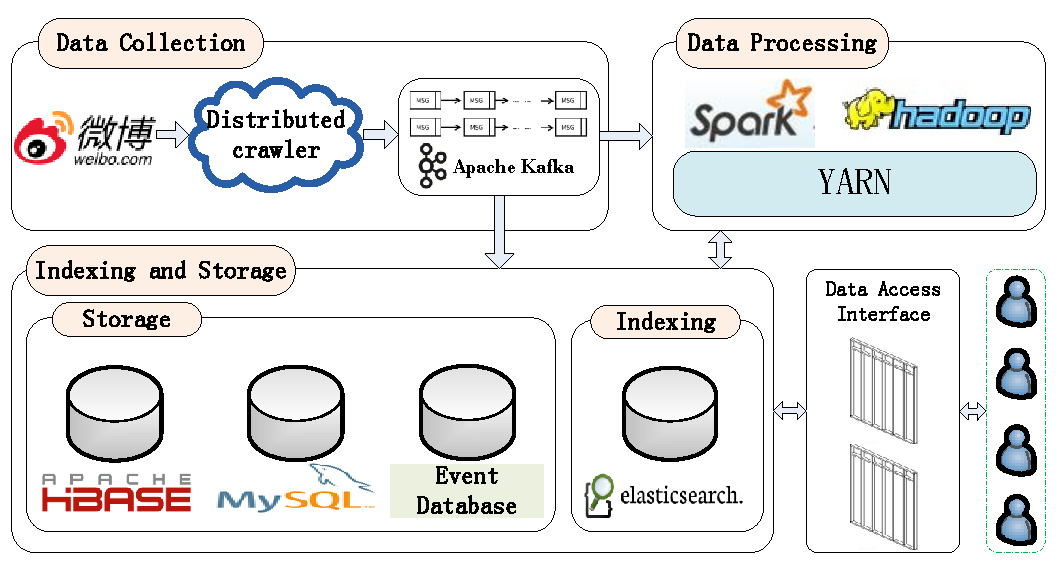
\includegraphics[scale=0.47]{system_architecture.pdf}
\centering
\caption{The Architecture of \ring System}
\label{fig:system_architecture}
\end{figure}

As shown in Figure \ref{fig:system_architecture},
\ring system mainly consists of three modules, namely data collection, data indexing \& storage and data processing.
%We implement a unified interface to process requests to these services.
For \emph{data collection}, we developed a distributed crawler to continuously fetch microblogs through Weibo API\footnote{http://open.weibo.com/wiki/Api}.
The collected data is forwarded to indexing and processing modules through Kafka\footnote{http://kafka.apache.org} to decouple their dependency.
For \emph{indexing and storage}, \ring utilizes HBase\footnote{http://hbase.apache.org/} and elasticsearch\footnote{https://github.com/elastic/elasticsearch} for data storage and full-text indexing, which is able to process large volumes of real-time microblog stream.
We further optimize elasticsearch over time range query for event tracking and query applications.
For \emph{data processing}, we implement our models and algorithms on Spark\footnote{http://spark.apache.org} and
 devise an optimization strategy for statistics incremental update to improve distributed processing efficiency.



%\subsection{Data Collection}
\noindent\textbf{Data Collection.}
We built a distributed crawler to collect data from Weibo, the largest microblog platform in China.
The crawler continuously collects the latest microblogs published by users preferrably with a large number of followers, \ie opinion leaders.
The crawler has a master/slave architecture.
The master node utilizes key/value store to perform task scheduling.
Slave nodes get the assignments from the master node and crawl data from Weibo.
A task would monitor the reposts and comments of an original tweet and retrieve the repost and comment list, 
from which we can construct the forward graph of each tweet message.
The tasks are scheduled according to posts' priority, which is weighed by the number of reposts and comments.
Each task has a life cycle so that each thread of post can be effectively monitored or terminated.
In order to make full use of computer resources and the limited API bandwidth, we deploy the crawler in KVM virtual machines.
The data is crawled using Weibo API in public privilege. 
Due to recent change on the public API, up to now we are able to collect 3 - 10 million microblogs daily.


\noindent\textbf{Indexing:}
%\subsection{Indexing}
\label{index}
We built our full-text index for microblog texts and the emerging events with elasticsearch.
Event evolution tracking application issues extensive amount of keyword queries to retrieve related tweets for similarity computation.
Each query is issued toward data in a specific time interval as defined in the event detection algorithm. 
We add a time range structure in the multi-layer index of elasticsearch to directly optimize time range query performance~\cite{huang2015indexing}.
Such structure for time ranged queries avoids traversing each layer and allows efficient navigation to records within a specified time interval.



%There are two important data structures for performance improvement:% in the indexing engine of \ring:
%\emph{Word Partition:}
%A word partition is an equal-length partition created by dividing the fixed dictionary in alphabetical order.
%Words of the text are hashed into different partitions and such a fine-grained partition strategy would improve index and query performance through better parallelization.
%%(What's the vocabulary? Is range dynamic?)
%%\textbf{Multi-Layers:}
%%Every partition is a multi-layered index. A threshold governs the size of each layer.
%%New data are first inserted into the lowest layer.
%%When it reaches the size threshold, the data of this layer would be moved to a higher layer in a batch manner.
%%This structure can obtain the tradeoff between index and query.
%%(Why do we do this? What's the old es way? How is the improvement/comparison?)
%\emph{Time Range:}
%Event tracing application and queries to microblog texts would require high performance time range queries.
%We add a time range structure in the multi-layer index of elasticsearch.
%Such structure for time ranged queries avoids traversing each layer and allows efficient navigation to records within a specified time interval.
%%Long time range queries could also be processed efficiently due to the multi-layer merging strategy.
%%(What does this mean?)

%%By using the above index structure, \ring can reduce the cost of traversing the index effectively.
%%The optimized index can index 2k microblogs per second compared to 1.2k in the same setting without optimization.
%%(What) Query latency is reduced by 50\% on average.
%%(How much improvement?)


\noindent\textbf{Distributed Processing:}
%\subsection{Stream Processing}
Our monitoring algorithms are implemented on Spark.
As discussed in Section~\ref{detection}, a continuously changing graph of keywords and their co-occurrence relationship is built from the text stream.
To improve the efficiency of graph update, we created an index in each partition of the Spark RDD to rapidly locate data records and enable fine-grained incremental updates~\cite{ju2015igraph}.
This alleviates the overhead of data copy and shuffling when updated nodes only account for a small portion of the graph and when updated statistics of each node can be computed from a known portion of data, \ie tweets containing certain keywords in our case.
Experiments show that our method has a speedup of 3.7X for incremental statistics update and 5.4X for incremental PageRank.

%(What's the performance improvement, by how much?)

%\textbf{Incremental Computing:} The data in each partition of RDD is divided into two parts, \textit{raw data part} and \textit{incremental data part}. The incremental data %part is structured by a sequence of blocks, each contains the update messages in a certain time interval. When all the computation tasks relying on some block have been %executed, the data in the block is merged into the raw data part.

%\textbf{Work Balance:} The computation cost of the hot spot during event detection is higher, often proportional to the heat rate. Upon recording such costly data in each %partition and evaluate its heat rate every period of time, we build an optimizing model to rebalance to make all the partitions approximately have total heat rate. According %to the result of the model, partitions exchange data and record this change to ensure the rightness of locating with the index.




%\subsection{Event Database}
As discussed in Section~\ref{detection} and~\ref{tracing}, the detected events and their corresponding storylines can be discovered by our system. With the accumulation of these information, the pattern of how events developed and how they are related can be generalized. To facilitate this pattern mining functionality, we create an event knowledge base for storing the collected data and design a set of pattern mining algorithms for infer the hidden dependencies between events.
\begin{figure}[h!]
\centering
\includegraphics[width=.48\textwidth]{ekbArchitecture}
\caption{Event Knowledge Base Architecture}
\label{fig:architecture}
\end{figure}

Specifically, we implement the event knowledge base as a two level graph structure. The first level directly stores the detected results (including events, storylines, and dependencies). The second level stores the generalized concepts and their sequential dependencies. The goal of the provided algorithms is to build the connection between these two levels and to detect the sequential pattern between concepts. In practice, the collected events are continuously accumulated. This dynamic characteristics of event streams requires the design of the pattern mining module capable of accommodating such dynamics and operating both effectively and efficiently.

Figure~\ref{fig:architecture} shows the architecture of Event Knowledge Base. The database consists of two modules: on-line module and off-line module. The low-complexity on-line module instantaneously saves the new arrived events into the knowledge base and invokes concept generalization algorithms to update the knowledge base. Off-line model contains pattern mining algorithms with relatively high computational cost and is called up both on demand.

%\section{System Architecture}
\section{Demonstration}
\makeatletter
\setlength{\@fptop}{0pt}
\makeatother

%\subsection{Overall Architecture}
\begin{figure}[!t]
\centering
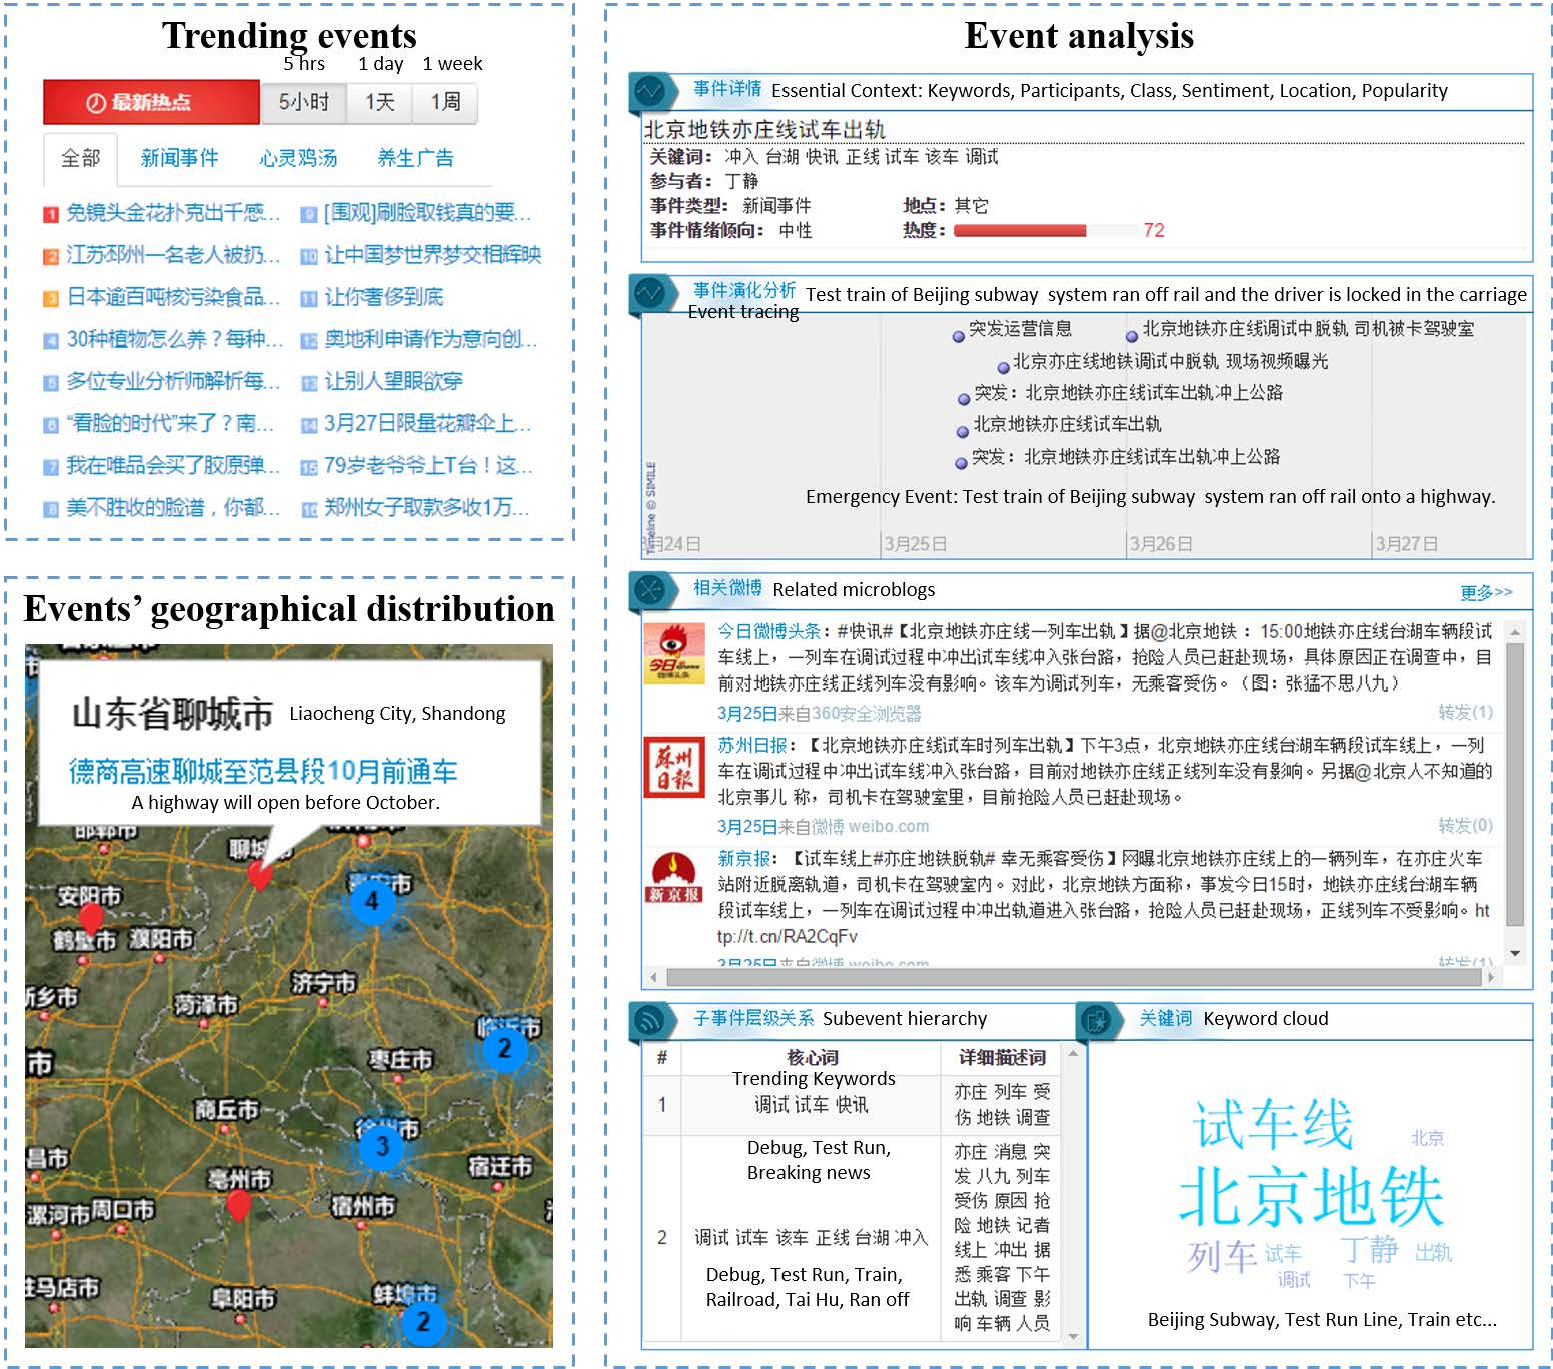
\includegraphics[width=3.3in, height=2.85in]{UI}
\caption{Features of Demonstration}
\label{fig:UI}
\end{figure}


%\subsection{User Interface}
\noindent\textbf{Features for Demo.}
We demonstrate three features based on emerging event monitoring algorithms, as shown in Figure \ref{fig:UI}.

\emph{Trending Event Ranking:}
%Events detected by \ring system are tracked based on the method mentioned in Section \ref{tracing}.
Events are ranked according to the volume of their related microblogs.
The ``hottest'' trending events in the past 5 hours, 1 day and 1 week are displayed on the front page of \ring system.
Our monitoring application could cover emerging events ahead of major news sites, \eg sina.com.cn or baidu.com.
Spam information has been effectively removed and missing events are majorly due to absence of data.
%There would be missing events

\emph{Event Analysis:}
Navigated from a search or the trending event ranking feature, the event analysis page shows detailed information of a detected event which includes representative tweet as human-readable abstract, time of detection, keyword summarization, participants, event class as news or spam, location, sentiment bias and popularity, etc.
The evolution of the current event is displayed on a timeline interface, together with related microblogs and sub-event hierarchy represented with ranked trending keywords.
A word cloud of frequent keywords in related tweets is also displayed.
Note that the trending keywords are not necessarily the most frequent keywords.

\emph{Geographical Distribution:}
The geographical distribution page shows a map with ballon markups indicating the number of events in the location.
Click on the ballons would display events in a specified location.
A search box allows users to query and navigate to the location more quickly.


\newcolumntype{C}{ >{\centering\arraybackslash} m{5.5cm} }
\newcolumntype{D}{ >{\centering\arraybackslash} m{1.8cm} }
\begin{table}
%\begin{minipage}[!t]{.5\textwidth}
%\raggedright
%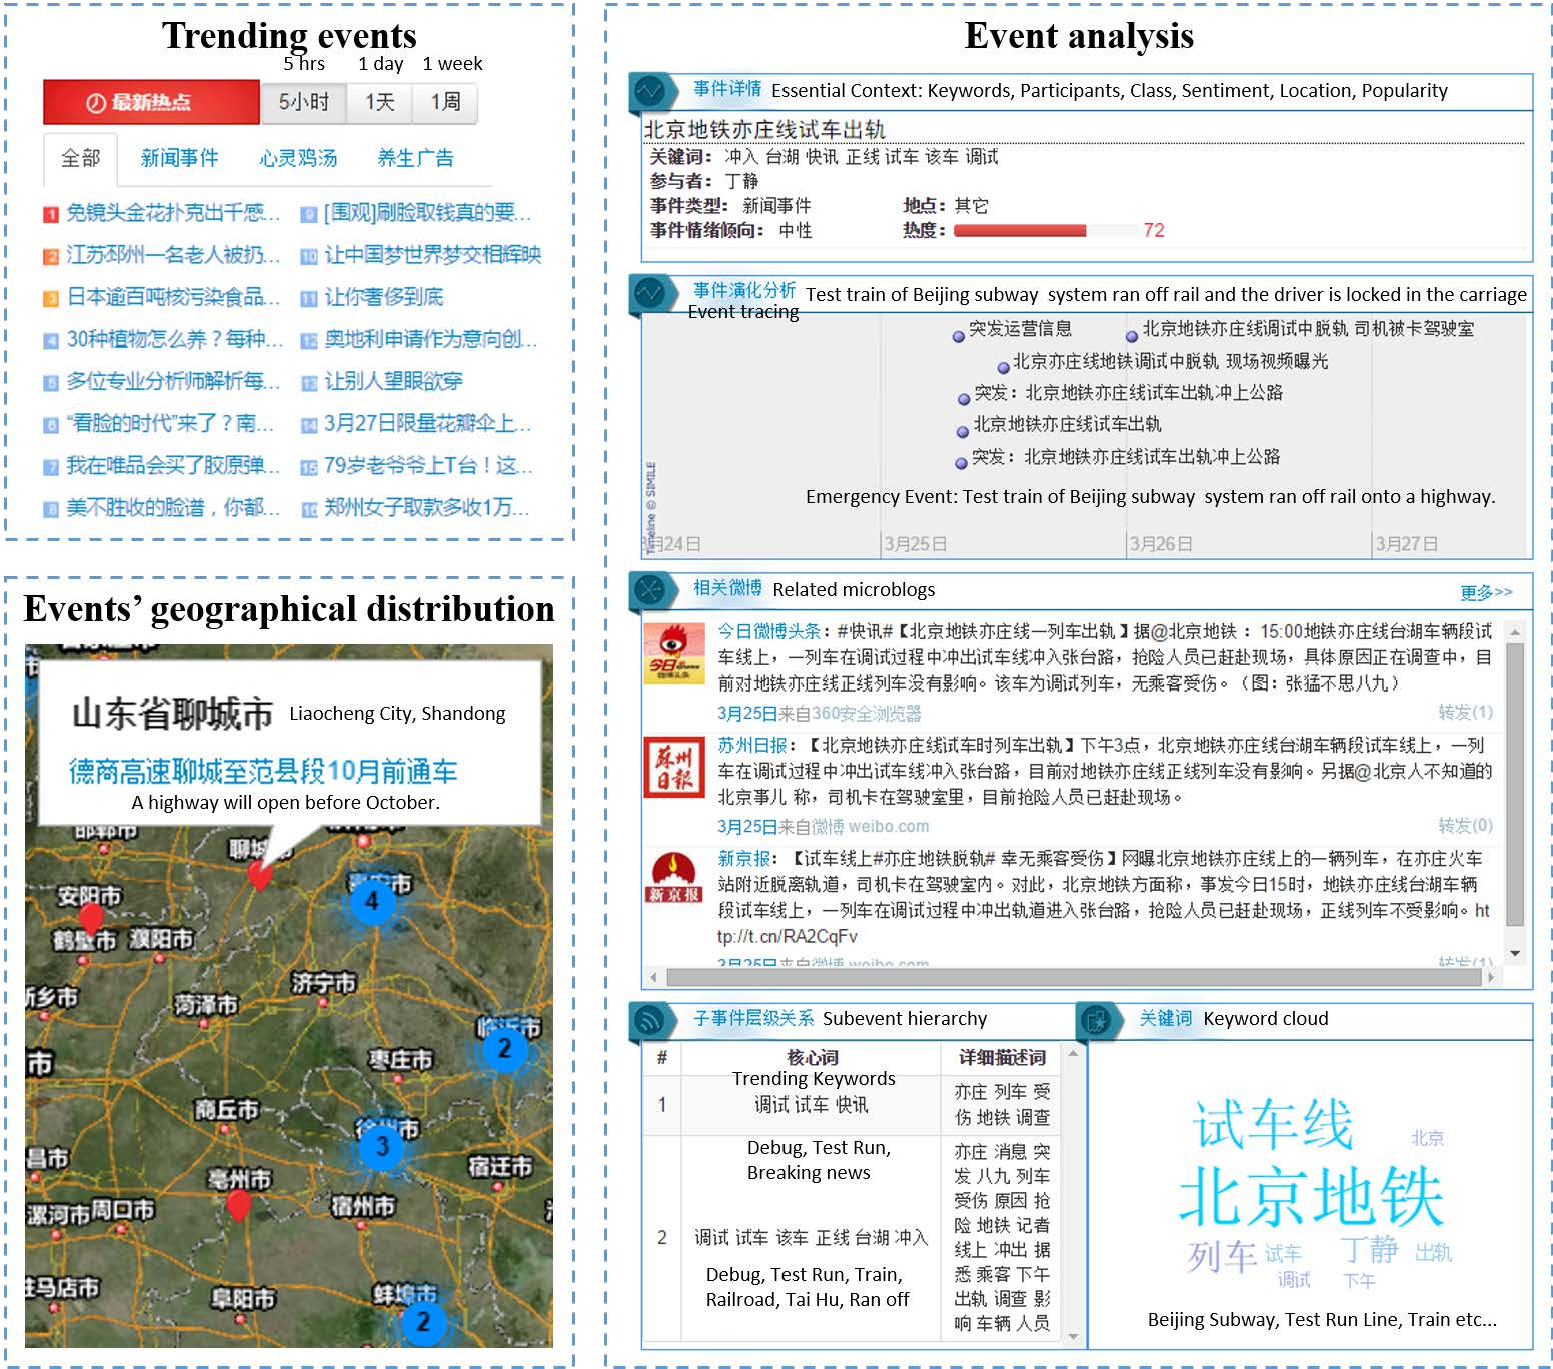
\includegraphics[width=3.3in, height=2.85in]{UI}
%\caption{Features for Demonstration}
%\label{fig:UI}
%\end{minipage}%\hfill
%\small
\raggedleft
\caption{A Case of Event Evolution Chain}
\begin{tabular}{|D|C|} \hline
\textbf{Time} & \textbf{Event description} \\ \hline
2014-12-01 18:40:00 & The suspect of Fudan poisoning case writes an apology letter to the victim's parents. $|$ The $2^{nd}$ trial will be held. \\ \hline
2014-12-08 08:10:00 & Fudan poisoning case's second trial will be held in 10am today, victim's parents will be in court. \\ \hline
2014-12-08 12:50:00 & LIVE: Defendant of Fudan poisoning case cries in court.\\ \hline
2015-01-08 07:40:00 & The court will pronounce judgement of the $2^{nd}$ trial today and victim's father hope to maintain the death penalty.\\ \hline
2015-01-08 10:30:00 & The court maintains the former death sentence on attempted murder in the second trail of Fudan poisoning case. \\ \hline
\end{tabular}
\label{fig:evolution}
\end{table}

\begin{table}
%\small
\raggedleft
\caption{A Case of Hierarchical Sub-Event}
\begin{tabular}{|D|C|}
\hline
\multirow{2}{1.8cm}{Poisoning Case, Fudan} & Apologize, Lin Senhao, Open a Court Session, Write \\ \cline{2-2}
                                           & Scheduled to, Shanghai \\ \hline
\end{tabular}
\label{fig:subevent}
\end{table}


%\subsection{Case Study}
\noindent\textbf{Case Study.}
\label{casestudy}
We demonstrate through case study the effectiveness of \ring for multi-granularity, multi-aspect event monitoring that it can tell the story of an event automatically.
An evolution chain distilled by \ring is shown in Table~\ref{fig:evolution}.
Given (by search or trending event ranking interface) the ``latest'' event in the table, an evolution chain that spans several month was revealed.
These events are about the second trial of the infamous poisoning case in Fudan University, China,
where the suspect poisoned his roommate to death in April 2013.
The detected events are all significant in its development and we can see that forecast, process and judgement of the trial all drew a lot of attention, hence detected by \ring.
The descriptions of these events are extracted automatically either directly from tweets or from representative tweets that contained predefined brackets indicating proper titles.
Recall from~\ref{detection} that our system reports trending events in 10-minute intervals.
Each of these events in Table~\ref{fig:evolution} has been repeatedly detected in consecutive time intervals, lasting from 20 minutes to 60 minutes.
It is indicated by trending keywords detection algorithm that a consecutive exponential growth of tweets in volume has been detected.
The system consolidate such similar events to show only one such event and highlight such event for special attention.
We manually inspect the average latency of detection of these events, i.e. the time from the first tweet appearing in our data to the detection time, to be 14.4 minutes, which is shown in the table.
%A event evolution case is shown in Figure \ref{fig:evolution}. All the events are detected using our method proposed in Section \ref{detection}.

%Our algorithm can trace all the developmental stages of this case's second trial as you can see from the table, even though they spans over several months.
The sub-event hierarchy of the first event in Table~\ref{fig:evolution} is shown in Table~\ref{fig:subevent}.
There are two aspects of the event.
The first is about the suspect writing an apology letter to the victim's parents and the other is that the second trial of the poison case is scheduled to be held in Shanghai, showing different aspects as history and current development of the event.




\section{Conclusions}
We demonstrate \ring, a \un{r}eal-t\un{i}me emerging eve\un{n}t monitorin\un{g} system over microblog platforms
that integrates our efforts from both event monitoring research and system research.
\ring can detect emerging events, build hierarchical sub-event correlation, trace event evolution and support queries to events and texts.
%Various optimization techniques have been developed to support efficient data processing and query.
\ring's infrastructure is equipped with optimized full-text search engine and distributed processing engine.
%To our best knowledge, \ring outperforms the state-of-the-art systems from both the semantic and systematic perspective.
The system present advantages over existing systems~\cite{xie2014clear, schubert2014signitrend, mathioudakis2010twittermonitor} from both the semantic and system perspective.








% ensure same length columns on last page (might need two sub-sequent latex runs)
\balance

%%ACKNOWLEDGMENTS are optional
\section{Acknowledgment}
This work is supported by grants from
the China 973 Fundamental R\&D Program (No.2014CB340300).



% conference papers do not normally have an appendix


% use section* for acknowledgement
\section*{Acknowledgment}


The authors would like to thank Zhongyu Lu, Haifei Huang, Chenggen Sun, Bo Wu and Xue Li for the help in setting up the system.
This work is supported by grants from the China 973 Fundamental R\&D Program (No.2014CB340300).





% trigger a \newpage just before the given reference
% number - used to balance the columns on the last page
% adjust value as needed - may need to be readjusted if
% the document is modified later
%\IEEEtriggeratref{8}
% The "triggered" command can be changed if desired:
%\IEEEtriggercmd{\enlargethispage{-5in}}

% references section

% can use a bibliography generated by BibTeX as a .bbl file
% BibTeX documentation can be easily obtained at:
% http://www.ctan.org/tex-archive/biblio/bibtex/contrib/doc/
% The IEEEtran BibTeX style support page is at:
% http://www.michaelshell.org/tex/ieeetran/bibtex/
%\bibliographystyle{IEEEtran}
% argument is your BibTeX string definitions and bibliography database(s)
%\bibliography{IEEEabrv,../bib/paper}
%
% <OR> manually copy in the resultant .bbl file
% set second argument of \begin to the number of references
% (used to reserve space for the reference number labels box)
%\begin{thebibliography}{1}

%\bibitem{IEEEhowto:kopka}
%H.~Kopka and P.~W. Daly, \emph{A Guide to \LaTeX}, 3rd~ed.\hskip 1em plus
%  0.5em minus 0.4em\relax Harlow, England: Addison-Wesley, 1999.

%\end{thebibliography}


% The following two commands are all you need in the
% initial runs of your .tex file to
% produce the bibliography for the citations in your paper.
\bibliographystyle{IEEETran}
\bibliography{Ring_Reference}  % vldb_sample.bib is the name of the Bibliography in this case
% You must have a proper ".bib" file
%  and remember to run:
% latex bibtex latex latex
% to resolve all references


% that's all folks
\end{document}


